\RequirePackage{ifpdf}
	\ifpdf	
		\documentclass[pdftex]{article}
		\RequirePackage{color} 
	\else
		\documentclass[10pt]{article} 
		\usepackage{nohyperref}		
	\fi

\usepackage[utf8]{inputenc}
\usepackage[T1]{fontenc}
\usepackage[left=1.5cm, top=1.3cm, textwidth=18.6cm, textheight=27cm]{geometry}
\geometry{paper=a4paper}
\usepackage{graphicx}
\usepackage{titling}
\usepackage{abstract}
\usepackage{fancyhdr}
\usepackage[procnames]{listings}
\usepackage{amsmath}

\definecolor{keywords}{RGB}{255,0,90}
\definecolor{comments}{RGB}{0,0,113}
\definecolor{red}{RGB}{160,0,0}
\definecolor{green}{RGB}{0,150,0}

\lhead{} \chead{} \rhead{}
\lfoot{\emph{Softcomputing, 2015/2016}} \cfoot{} \rfoot{\thepage}
\renewcommand{\headrulewidth}{0pt}
\renewcommand{\footrulewidth}{0.4pt}
\pagestyle{fancy}

\pretitle{
\includegraphics[width=.55\textwidth]{eka-en.png}\par\vspace{1ex}\begin{center}\huge}

\posttitle{\par\end{center}}
\preauthor{\begin{center} \large \begin{tabular}[t]{c}}
\postauthor{\end{tabular}\par\end{center}}
\predate{} \postdate{}
\date{}

\newcommand{\eng}[1]{(ang.\ \emph{#1})}

\title{\vspace{10ex} Softcomputing report \\ \vspace{6ex} Thermal pictures of human faces recognition by \\ Kohonen Neural Network \vspace{32ex}}

\author{Maciej Borkowski\\ 195968@student.pwr.edu.pl}

\begin{document}
\thispagestyle{empty}
\maketitle

\clearpage
\section{The problem}
In the problem we are given a set of real thermal photos of human faces. Each picture is of the same size and consists of a unique person's face and possibly some other parts of person's head or body that were also included in the shot (e.g. hair, ears, neck, background). The goal is to recognize pictures of the same person even when it is not the same photo, but the same person in different situations, the could very easily happen in real life situations, e.g. the person's temperature has changed, the shot has been taken from a different angle, part of the face is hidden behind some object.

 To accomplish this task test data has been found and adjusted, Kohonen's neural network has been implemented and parametrized accordingly to the test data and finally test have been run in order to investigate and analyse the suitability of such solution in real life situations.

\section{Kohonen's neural network introduction}
Artificial neural networks have been studied and
helped in the development of information processing models based on or inspired by biological
neural structures for a long time now. Not only can they provide solutions with improved
performance when compared with traditional problem-solving methods, but
also give a deeper understanding of the inner workings of living being's brains. Among various
existing neural network architectures and learning algorithms, Kohonen’s self-organizing
map (SOM) is one of the most popular neural network models.  Although
the computational form of the SOM is very simple, numerous researchers
have already examined the algorithm and many of its problems, nevertheless
research in this area goes deeper and deeper – there are still many aspects to
be exploited. Modeling and analyzing the mapping are important to understanding how the brain
perceives, encodes, recognizes and processes the patterns it receives.

Developed for an associative memory model, Kohonen's network it is an unsupervised learning
algorithm with a simple structure and computational form, and is motivated
by the retina-cortex mapping \cite{kohonen}. Self-organization in general is a fundamental
pattern recognition process, in which various pattern relationships
among the stimuli and responses are learnt without the presence
of a potentially biased or subjective external influence (i.e. a teacher). The Kohonen technique creates a network that stores information in such a way that any topological relationships within the training set may be maintained.

\section{Learning and testing data sets}
\subsection{Learning data}
The thermal images of human faces are a part of  IRIS Thermal/Visible Face Database \cite{dataset}. The part, which was used in the task consists of thermal images images of people from different perspectives taken at, what seems to be, nearly the same moment. Nine images of different people, which did not had eyeglasses during photo taking, have been chosen as the learning set. These images are taken straight from the front of the person. These images had been preprocessed by cutting a 128x160 rectangle from each, that represents the face and as little other things as possible (Figure \ref{faces}).
\begin{figure}[!htb]
	\centering
	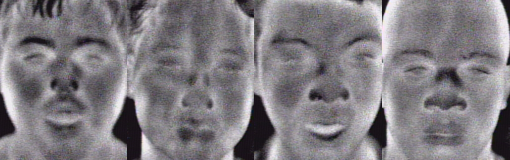
\includegraphics[width=0.85\textwidth]{pictures/faces.png} 
	\caption{Four example faces taken from the learning data set}
	\label{faces}
\end{figure}

\subsection{Test data}
The test data was obtained using a few methods:
\begin{itemize}
\item{the use of photos of the same people from different angles from the same database}
\item{simple manually created changes to available faces using image processing tool}
\item{brightening and darkening of image imitating respectively heating up and chilling down person's skin}
\end{itemize}

\clearpage
\section{Implementation}
\subsection{Environment}
An application in Java was written implementing the Kohonen's neural network from scratch with tuneable parameters.
\subsection{Initialization}
The assumption is that the data has been preprocessed and each thermal photo is available as a grayscale image, in which each pixel corresponds to one value between 0 and 1. The initialization phase starts with normalization of the inputted learning data, so that the sum of it's pixel values equals one:
$$ x_i^* = {x_i \over \sqrt{\sum_{a}^{n} x_a^2}} $$
Then, the neural net is initialized. A two dimensional net, with parametrised side lengths. Each neuron in the nethas it's own weights assigned to each of the input image pixel values. The value of the weights is initialised between values $-1$ and $1$ with uniform distribution.
\subsection{Learning}
The learning phase consists of multiple steps done in a loop, each on all of the inputted learning data, for a parametrized number of times. Each time winner neurons are found and then their, possibly with some neighbourhood neurons', weights are approprietly updated. The learning steps:
\begin{enumerate}
\item{Update parameters} \\
Two essential parameters are updated in this phase and later used to update network's weights:
\begin{itemize}
\item{Learning rate} \\
Decreases linearly from it's maximum value to it's minimum value (parameters).
\item{Mexican hat parameter} \\
Increases linearly from it's minimum value to it's maximum value (parameters).
\end{itemize}
\item{Shuffle learning data} \\
The data set is shuffled so that the images are shown in random order each time.
\item{Find winners} \\
For each image a winner has to be found amongst the neurons, that create the neural net. Each neuron can be the winner for only one image in the loop rotation. In case a neuron is already a winner for another image, the it is ignored, and the second best fit is declared a winner. Winner neuron is the one that is the closest to the the input image vector. The proximity between a neuron and image is defined as the euclidean distance between neuron's weights and image vector values:
$$ D = \sqrt{\sum_{j=1}^{N} (x_j-w_j)^2} \;, where $$
$$ x-input\; image $$
$$ w-neuron's\; weights $$
\item{Apply Grossberg Rule} \\
For each winner neuron from previous step is used to scan the whole net accordingly updating the weights of those neurons, based on the proximity to the winner neuron:
$$ w_{ij}^* = w_{ij} +  \eta  h(i^w, j^w, i, j)(x - w_{ij}) \; , \; where $$
$$  i,j-neuron's \; coordinates $$
$$  w-neuron's\; weights $$
$$ \eta-learning\; rate $$
$$ x-input\; image $$
$$ h(i^w, j^w, i, j) =
 \begin{cases}
 1  			& \quad \text{if } r=0\\
 sin(ar) \over ar 	& \quad \text{if } r \in ({0, {\pi \over a}})\\
 0  			& \quad \text{otherwise} \\
  \end{cases}$$
$$ r-euclidean \; distance \; between \; neurons \; of \; coordinates \; (i,j) \; and \; winner \; neuron \; (i^w,j^w) $$
$$ a-mexican \; hat \; parameter$$
\end{enumerate}
\subsection{Retrieval}
After learning phase the network is ready to give us output for a new input image. The return value for each neuron is calculated:
$$ y=\sum_{j=0}^{N}x_jw_j $$
Neurons with the higher output values give us better response to the stimuli. Two input images with the best responses in similar neurons are recognized as similar images.
\subsection{GUI}
A graphical user interface has been created to easily change change some parameters of network, visually represent the output of neural network on a given stimuli and to brighten or darken the input image simulating a change in temperature (Figure \ref{gui}).
\begin{figure}[!htb]
	\centering
	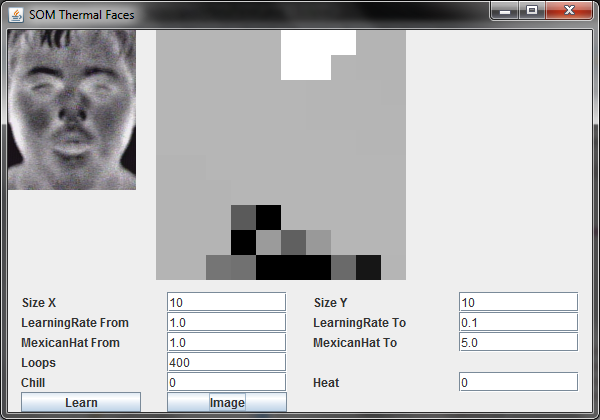
\includegraphics[width=0.85\textwidth]{pictures/gui.png} 
	\caption{Graphical User Interface}
	\label{gui}
\end{figure}
Using the GUI user can:
\begin{itemize}
\item{set the size of the network}
\item{set the range of learning rate}
\item{set the range of mexican hat ($sinc$ function) parameter}
\item{set the number of loops in learning phase}
\item{start learning phase with chosen parameters}
\item{set the percentage of chilling down or heating up the image}
\item{choose image to stimulate created network}
\item{see the chosen input image after optional chilling or heating its temperature}
\item{see the visual representation of the neural network, where each neuron is shown as a square with color ranging from black (smallest response) to white (biggest response)}
\end{itemize}

\section{Results analysis}
\subsection{Reliability}
The learning process is not always reliable. Often, in about 25\% cases, only a smart part of the neuron net will be used and the net will respond similarily to any stimuli, giving us no information. This seems to be independent on the number of loops. Creating a new network with the same parameters can help in these situations. It should be possible to check for these situations automatically and build a new net each time.
 
\subsection{Tuned parameters}
Experimentally, the parameters of the network have been tuned in such a way that the network returns usable responses from the map using the map's response visual representation. For the nine input images used a network of 10x10 neurons is used. In each of 400 loops all input images stimulate the network. With every loop rotation, the learning rate is decreased linearly from $1.0$ to $0.1$ and parameter used in mexican hat ($sinc$ function) increases from $1.0$ to $5.0$, which corresponds to the change of accepted neighbourhood distance from slightly more than the radius of $3$ (Winner Takes Most) to the radius of less than $1$ (Winner Takes All). For such parameters the learning process takes about 30 seconds.

\subsection{No change}
When there is not change involved in the input pictures, meaning that the same pictures that were used in the learning procedure are used now, then there network's response is very reliable and the network distinguishes between people, by assigning each to a few  neurons, that are close to each other, making a person stimulate part of the visual map (Figure \ref{nochange}). 

\begin{figure}[!htb]
	\centering
	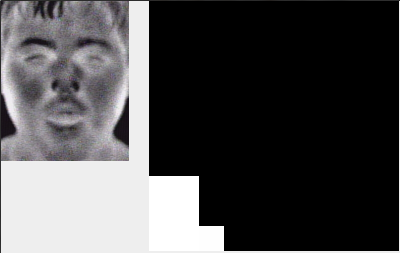
\includegraphics[width=0.45\textwidth]{pictures/nochange.png} 
	\caption{The network gives a strong response in neurons located in the lower left corner}
	\label{nochange}
\end{figure}

\subsection{Temperature}
\subsubsection{Global}
To imitate a global change in temperature, the image is accordingly darkened or lightened. In this case of lightening up the completely black parts are not lightened at all, because it's assumed that background and hair does not change temperature much and we really care about changing the temperature of the skin.

When the temperature is decreased or increased on the whole image, the network's response does not change at all (Figures \ref{chill} and \ref{heat}).
\begin{figure}[!htb]
	\centering
	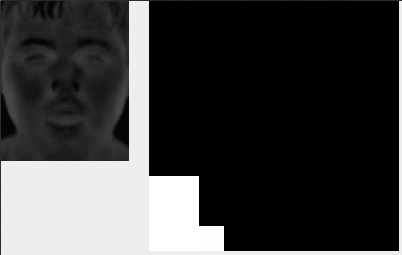
\includegraphics[width=0.45\textwidth]{pictures/chill.png} 
	\caption{Decreased temperature}
	\label{chill}
\end{figure}
\begin{figure}[!htb]
	\centering
	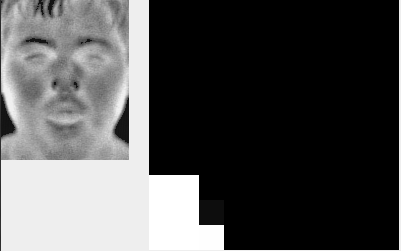
\includegraphics[width=0.45\textwidth]{pictures/heat.png} 
	\caption{Increased temperature}
	\label{heat}
\end{figure}

\subsubsection{Partial}
To imitate a partial change in temperature, an image processing tool has been used to lighten up parts of a face including mostly nose and cheeks(Figures \ref{part1} and \ref{part2}). In real life situation this could happen in winter, when some parts of face are more heated up than normally. Even for a big, but still reasonable amount of temperature increase the network's response still produced a response that enables us to easily recognize the person.

\begin{figure}[!htb]
	\centering
	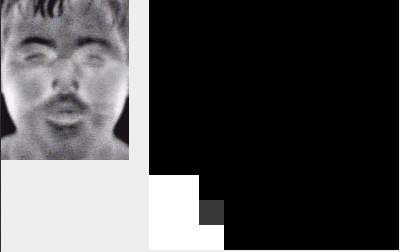
\includegraphics[width=0.45\textwidth]{pictures/part1.png} 
	\caption{Small, partial temperature increase}
	\label{part1}
\end{figure}
\begin{figure}[!htb]
	\centering
	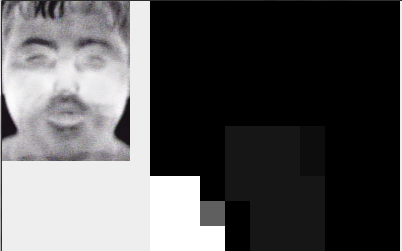
\includegraphics[width=0.45\textwidth]{pictures/part2.png} 
	\caption{Big, partial temperature increase}
	\label{part2}
\end{figure}

\clearpage
\subsection{Head rotation}
When a person's head is rotated the network's response can quickly become unreliable. The bigger the angle is the worse the reponse given by network. However for small changes in the angle of the taken photo the person is still recognized by the network (Figure \ref{rot}).

\begin{figure}[!htb]
	\centering
	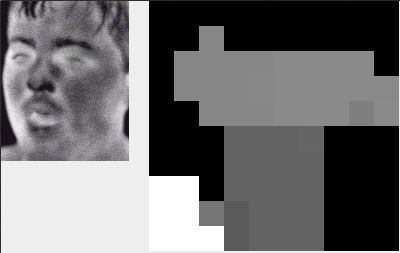
\includegraphics[width=0.45\textwidth]{pictures/rot.png} 
	\caption{Head rotated right}
	\label{rot}
\end{figure}

\subsection{Hidden faces}
To imitate an object that a person has on his or her head, black parts have been introduced to the pictures. Imitations of a scarf and a winter cap were used (Figures \ref{cap} and \ref{scarf}). This generally results in more gray parts of the visual representation of the map, but the most important, white part is still left unchanged, which shows that the recognition of the face is still correct. 

\begin{figure}[!htb]
	\centering
	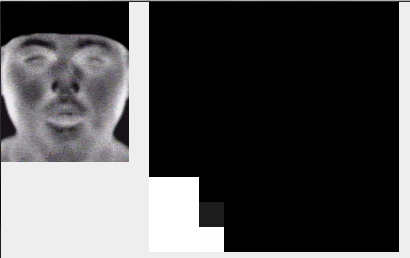
\includegraphics[width=0.45\textwidth]{pictures/cap.png} 
	\caption{Head with a winter hat}
	\label{cap}
\end{figure}
\begin{figure}[!htb]
	\centering
	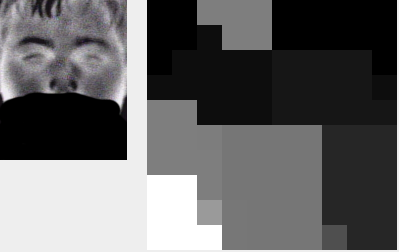
\includegraphics[width=0.45\textwidth]{pictures/scarf.png} 
	\caption{Head with a scarf}
	\label{pictures}
\end{figure}

\clearpage
Even after introducing both cap and scarf, effectively decreasing the size of meaningful part of picture to less than 50\% the face is still recognized (Figure \ref{capscarf}).

\begin{figure}[!htb]
	\centering
	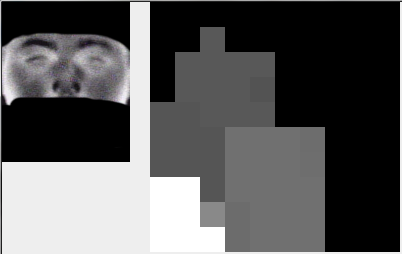
\includegraphics[width=0.45\textwidth]{pictures/capscarf.png} 
	\caption{Head with both a winter hat and a scarf}
	\label{capscarf}
\end{figure}

\subsection{Mixed changes}
\subsubsection{Winter hat and increased temperature}
Using the above mentioned possibilities some more complicated changes to the pictures can be created by mixing them together. Such cases are probable to occur in real life situations. For example a person in cold weather can have both heated up skin and a winter hat on head. In such case the person should still be recognized (Figure \ref{heatcap}).

\begin{figure}[!htb]
	\centering
	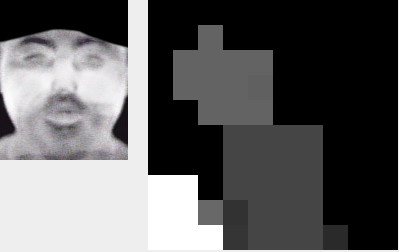
\includegraphics[width=0.45\textwidth]{pictures/heatcap.png} 
	\caption{Head with winter hat and partially increased temperature}
	\label{heatcap}
\end{figure}

 If such picture is additionally taken from an angle the person is barely recognizable and the response is not very reliable, but in most cases it will recognize the person correctly (Figure \ref{rotheatcap}).
\begin{figure}[!htb]
	\centering
	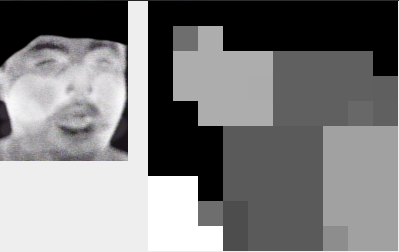
\includegraphics[width=0.45\textwidth]{pictures/rotheatcap.png} 
	\caption{Rotated fead with winter hat and partially increased temperature}
	\label{rotheatcap}
\end{figure}

\clearpage
 In the most extreme case however, when this person additionally uses a scarf, the network becomes very unreliable and will give wrong answers more often than not (Figure \ref{rotheatcapscarf}).
\begin{figure}[!htb]
	\centering
	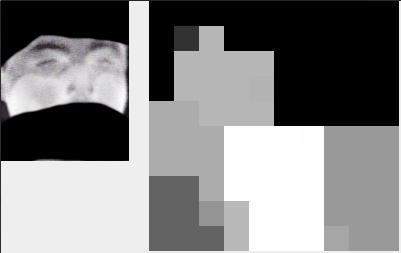
\includegraphics[width=0.45\textwidth]{pictures/rotheatcapscarf.png} 
	\caption{Rotated fead with winter hat, scarf and partially increased temperature}
	\label{rotheatcapscarf}
\end{figure}

\section{Final remarks}
To sum up, the Kohnen neural network worked well when recognizing human faces from thermal pictures from used dataset, when temperature was changed or part of the picture was hidden. Out of the analyzed changes to faces person's head rotation has the biggest impact on network's recognition reliability. Unfortunately this is probably also one of the most common changes, we could see in real life scenarios. A possible way to fix or at least reduce this problem could involve a much bigger learning set, containing multiple faces of the same person taken from similar angles and then fiddling with all the parameters so that these pictures trigger neurons which are close to each other, which would really make use of of Kohonen network's properties. This however requires a lot of computational power, because the learning set would have to be increased greatly, similarly the number of neurons and probably the number of loops for the learing phase. Generally, the bigger the amount of people, the network has to be able to recognize, the bigger the amount of time needed for learning phase.

 \begin{thebibliography}{1}
\bibitem{kohonen} Kohonen T (1982) {\em Self-organised formation of topologically correct feature
map. Biological Cybernetics}, 43: 56–69.
\bibitem{dataset} Besma Abidi {\em IRIS Thermal/Visible Face Database} http://vcipl-okstate.org/pbvs/bench/index.html 2015/12/12
\end{thebibliography}

\end{document}
